%Correct the file name.
%X: book number
%Y: part number
%ZZZ: page number in three digits. So page 3 would be 003.

\documentclass[11pt]{amsbook}

\usepackage{../HBSuerDemir}	% ------------------------
\usepackage{graphicx}
\begin{document}

% ++++++++++++++++++++++++++++++++++++++
\hPage{b1p2/242}
% ++++++++++++++++++++++++++++++++++++++
any other row (column), the sum D' of the products thus obtained is zero.
\begin{proof}
	The expansion of D with respect to the $j^{th}$ column is  
	\begin{center}
		D = $ a_{lj}  C_{lj} + ...+ a_{nj} C_{nj}  $,
	\end{center}
	and
	\begin{center}
		D' = $ a_{lj} C_{lj} $ +...+ $  a_{nj} C_{nj}$  $ \Longrightarrow D' =$
		$\begin{vmatrix}
			... & a_{lk}&... & a_{lk}&...\\ 
    			& \vdots&    &\vdots&   \\
			...&a_{nk}&...&a_{nk}&...  \notag
		\end{vmatrix}$
		= 0
	\end{center}
by the Corollary of Theorem 2.
\end{proof}



% =======================================
%\section{aaaah}

%u




% =======================================
%\subsection{bbb}





% =======================================
\subsubsection{Rule of Sarrus:}
	For determinants of order 3 and \textit{only for these}, there is a rule for evaluation commonly used in practice. This rule of SARRUS  consists of rewriting the first two rows below the 		third one, and then multiplying the three elements on the main diagonal, multiplying those just below these elements and multiplying three others below the latter, and then obtaining 		the sum of these three products; next doing the same for the elements of the secondary diagonal and related ones, obtaining a second sum of three products. Then the difference 		between the first and second sum gives the value of the determinant:
	\begin{flushleft}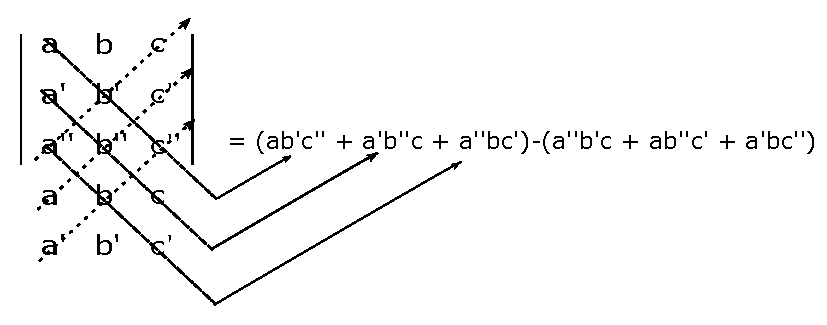
\includegraphics[width=1.0\textwidth,keepaspectratio=true]{images/b1p2-242-fig01}\end{flushleft}
\quad 
The rule is applied also by rewriting the first two columns after the third one.

%This is the first figure. 
%\begin{figure}[htb]
%	\centering
%	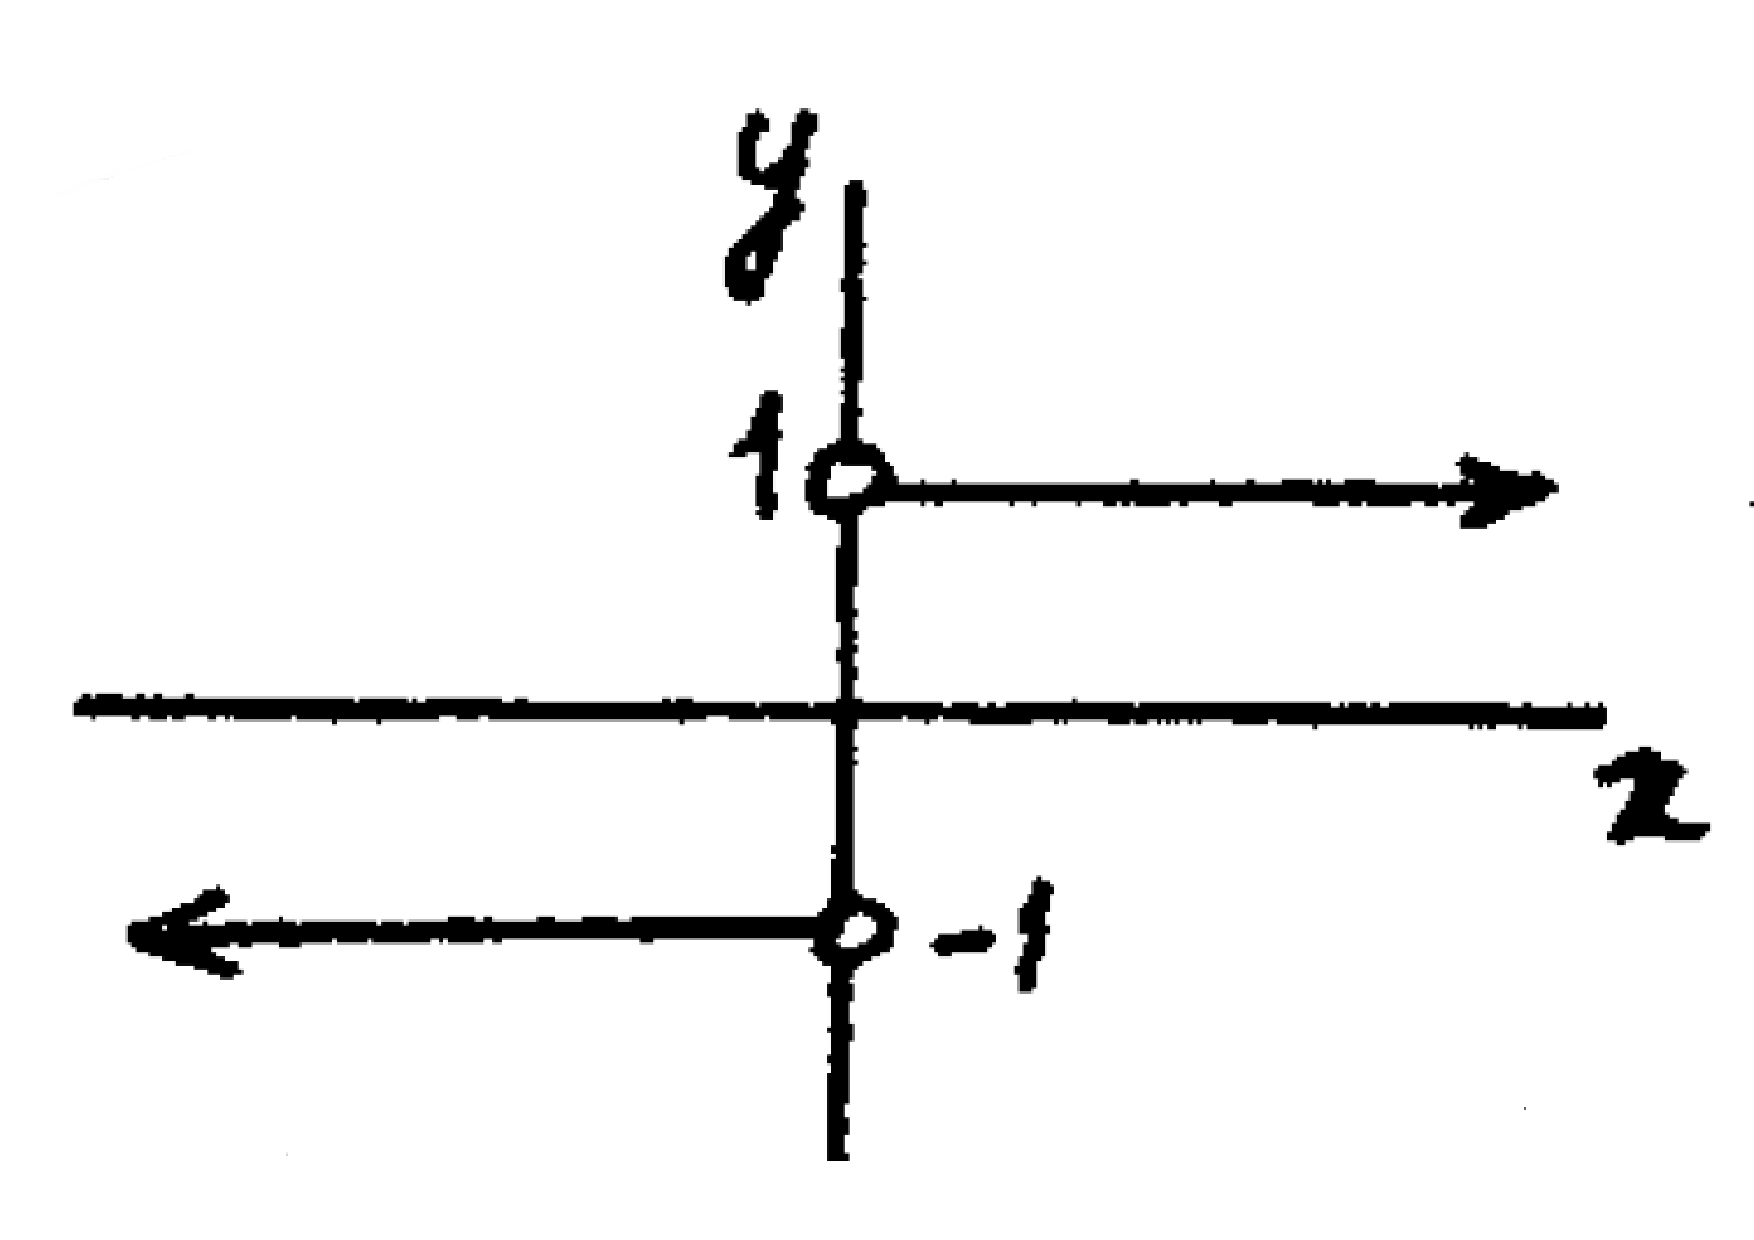
\includegraphics[width=0.45\textwidth]{images/bXpY-ZZZ-fig01}
%	\caption{Classification of complex numbers}
%	\label{fig:classificationOfComplexNumbersA}
%\end{figure}
%This is the second figure
%\begin{figure}[htb]
%	\centering
%	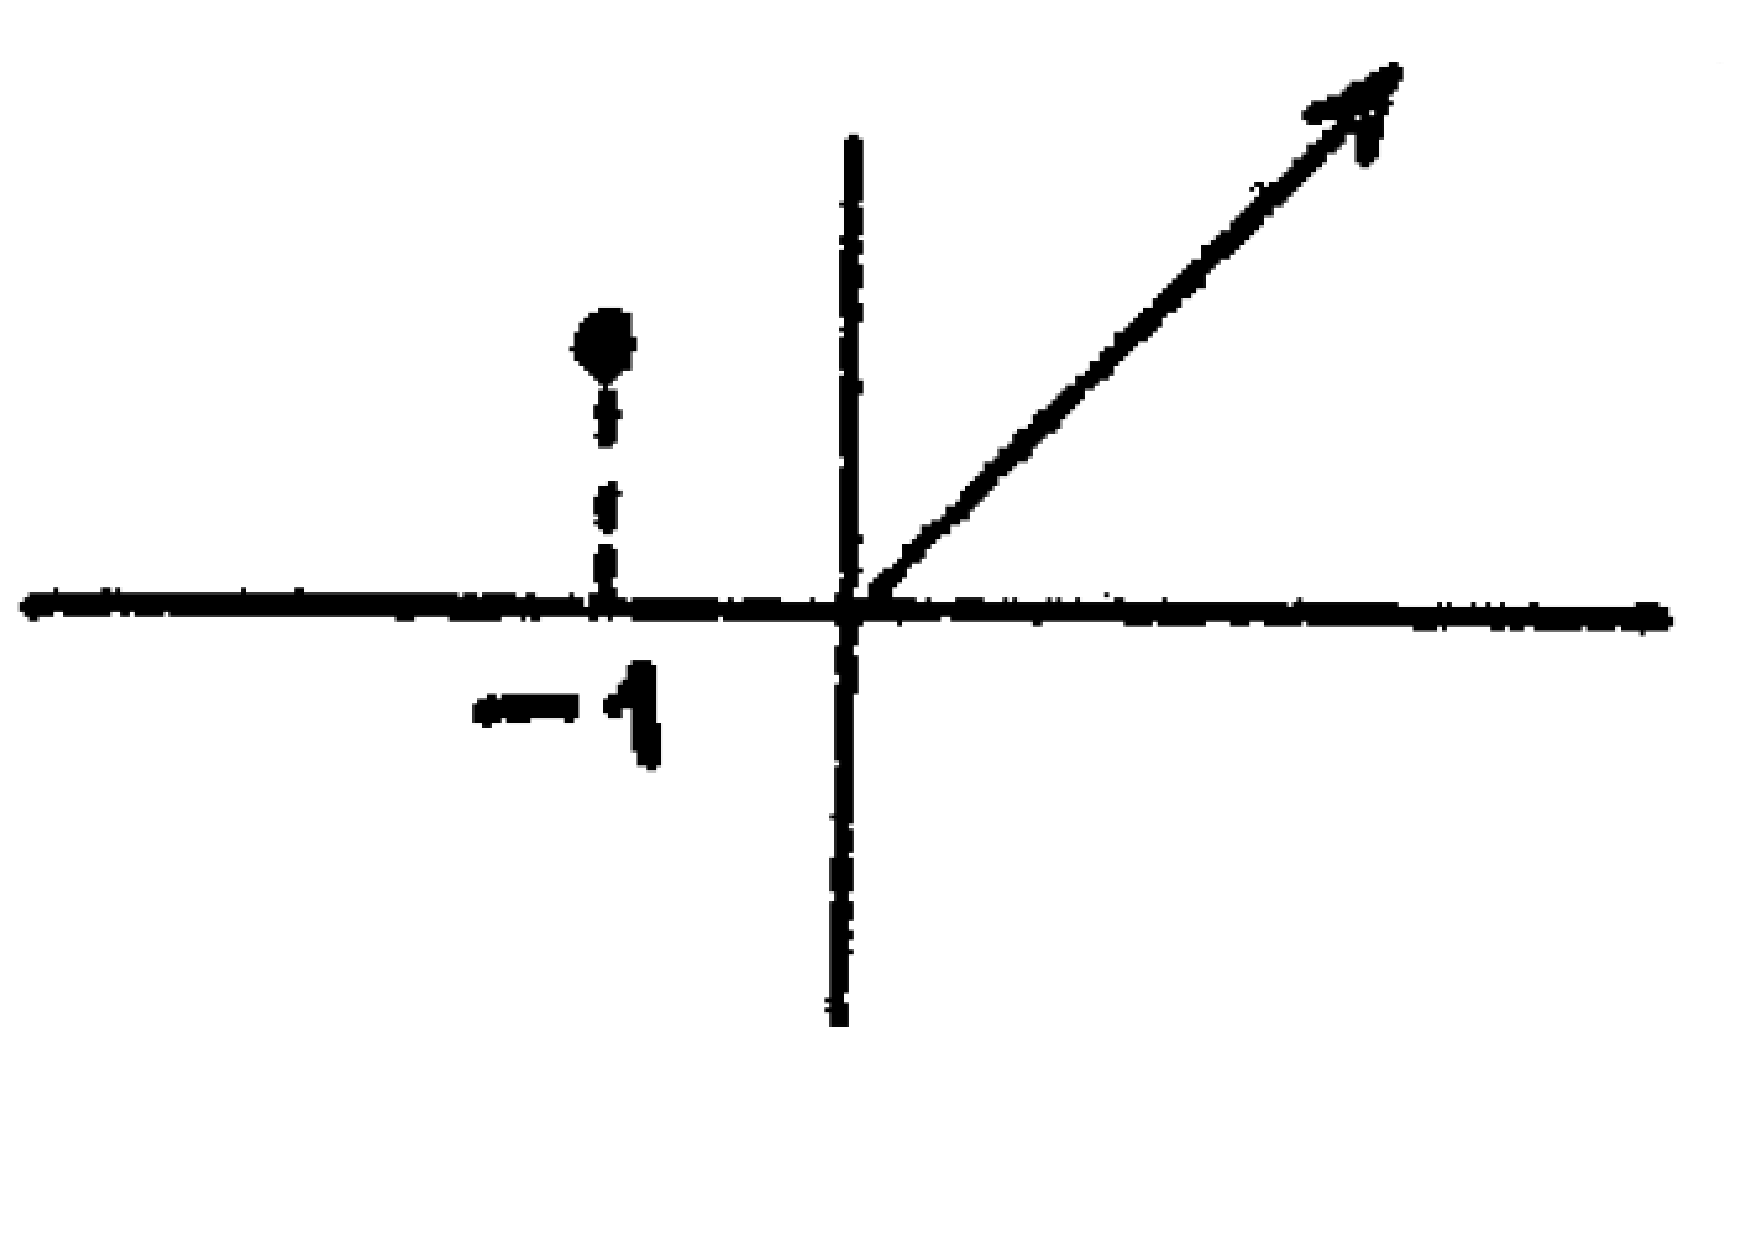
\includegraphics[width=0.45\textwidth]{images/bXpY-ZZZ-fig02}
%	\caption{Classification of complex numbers}
%	\label{fig:classificationOfComplexNumbersA}
%\end{figure}






% =======================================================
\end{document}  

%==== templates ====

%==== environments ====

%\begin{figure}[htb]
%	\centering
%	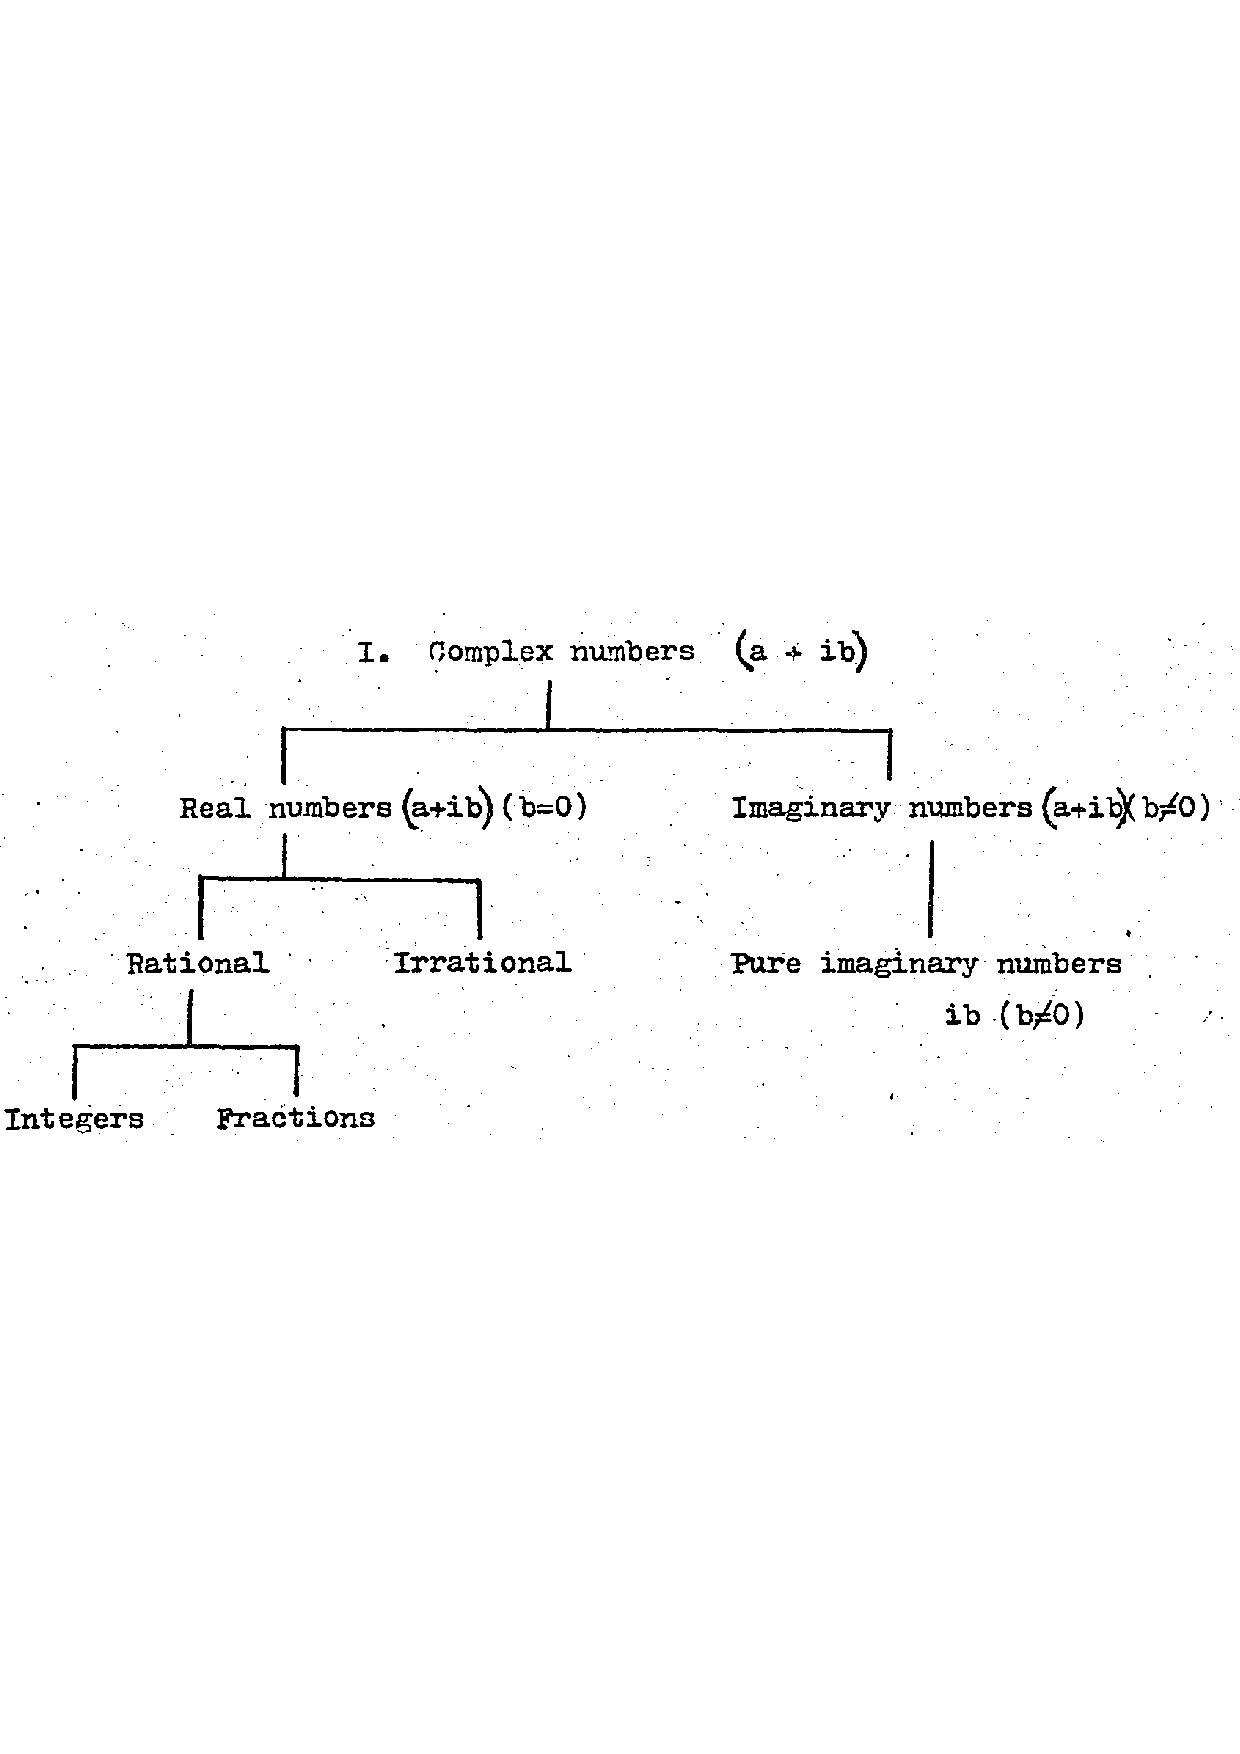
\includegraphics[width=0.9\textwidth]{images/SD-1-1p15A}
%	\caption{Classification of complex numbers}
%	\label{fig:classificationOfComplexNumbersA}
%\end{figure}

%\begin{center}
%\begin{tabular}{cc}
%\end{tabular}
%\end{center}

%\begin{exmp}
%\begin{hSolution}
%\end{hSolution}
%\end{exmp}

%\begin{hEnumerateAlpha}
%\end{hEnumerateAlpha}

%\begin{hEnumerateRoman}
%\end{hEnumerateRoman}

%$
%\begin{bmatrix}
%\end{bmatrix}
%$

%\frac{aaaa}{bbb}
%\frac{a_{n}}{b_{n}}
%\left( aaaa \right)
%\Longrightarrow

%\begin{multicols}{2}
%	bb
%\columnbreak
%	aa
%\end{multicols}
